\documentclass[11pt]{article}
%\renewcommand\refname{ }

\usepackage{fullpage}
\usepackage{epsfig}
\usepackage{graphicx}
\usepackage{listings,color}
\usepackage{mdframed}
\parskip=10pt

\input macros.tex

\definecolor{quotegray}{gray}{0.9}
% \lstnewenvironment{referee}{%
%   \lstset{backgroundcolor=\color{quotegray},
%   frame=single,
%   framerule=0pt,
%   basicstyle=\ttfamily,
%   columns=fullflexible}}{}

% https://tex.stackexchange.com/questions/111065/quoting-styles-technical-an-appreciation-questions
\mdfdefinestyle{myquotestyle}{
  leftmargin=15pt,
  rightmargin=15pt,
  backgroundcolor=quotegray,
  linewidth=0pt,
  skipbelow=\topskip,
  skipabove=\topskip
}
\newenvironment{referee}[1][]{%
    \ignorespaces%
    \begin{mdframed}[style=myquotestyle,#1]%
}{%
    \end{mdframed}%
    \ignorespacesafterend%
}%

% \newenvironment{referee}[1][]{
%   \ignorespaces%
%   \begin{mdframed}[style=myquotestyle,#1]%
% }{%
%   \end{mdframed}%
%   \ignorespaceafterend%
% }%



\begin{document}

\begin{center} 
\bfseries{
\begin{large}
  Response to referee report for manuscript ref. MN-19-2054-MJ
\end{large}
}
\end{center}

We thank the referee for their insightful review.  Their review is directly quoted below in the gray boxes with our responses below.  Any changes to the manuscript has been \textbf{bold-faced}.

\begin{referee}
The paper presented here is very well written and offers important new insights.  It studies the dependence of the halo mass for first star formation on a Lyman-Werner background in a large simulation, and goes beyond current literature work by the inclusion of self-shielding and studying the multiplicity of Pop III stars. I generally recommend if for publication after some concerns are addressed.
\end{referee}


\begin{referee}
Major comments:

1) One of the main points of the paper is studying the multiplicity of Pop III stars in a halo. This multiplicity might be due to the fact that Pop III stars have collapsed to a BH after their lifetime and a second Pop III star could form in the same halo. This is very plausible. If several Pop III stars are found forming in the same halo at the same time, however, the employed star particle algorithm has a hard-coded length scale of 1pc in which only one star particle can be formed. I am wondering if this is an effect that is resolution dependent - do the same number of stars form if the resolution is increased and the maximum distance is decreased? Which is the motivation for the length scale of 1pc?
\end{referee}

There was an error in the original draft of our paper, stating that "If within 1 pc, multiple cells meet this criteria, then a single Pop III star forms at the center of mass of these cells." It should instead say "within 10 pc", not "within 1 pc". This error has been corrected.

The 10 pc quoted above is a parameter called StarClusterCombineRadius, and controls how many stars form within a certain spatial range. Within our original simulation, this parameter was set to 10 pc, meaning that all stars younger than 10 kyr and within 10 pc of each other are merged into a single star. To make sure that this value does not affect our results, we have run simulations for a range of this parameter, namely from 0.625 pc to the original 10 pc. The simulations are a 1 comoving Mpc$^3$ box, zoomed-in on a single halo with a mass of $10^{7.7} M_{\odot}$ at the end of the run. The simulations run for a total of 10 Myr. We see the same number of Pop III stars form regardless of the chosen value for the merging parameter. Thus, our results are independent of this value. This detail has been added to section 2.2.1.


\begin{referee}
2) The authors select their haloes by the halo finding algorithm Rockstar. They should add a bit of information on that code (is it fof or subfind-like?). Also, one of their main points is to compare their work to Machacek+01. Machacek+01, however, use a different halo definition (spherical around the halo centre going out to a radius of 200 times the mean density of the Universe). How do these different halo masses compare?

Further, it is not entirely clear why atomic cooling haloes are excluded in this analysis and if they are excluded throughout the whole paper. The exclusion of atomic cooling haloes artificially shifts the average halo mass to lower values.

In addition, the authors should state the fraction of haloes that have Pop III stars forming outside the halo. The baryon fraction varies with redshift. Please give an estimate by how much this influences the halo masses used here.
\end{referee}

A short description of Rockstar has been added in section 3.1, where Rockstar is introduced.

We have compared the mass calculations between Rockstar and Machacek+01 and have found the following results. Figure \ref{fig:compare_mass} below shows how the Rockstar halo masses and the Machacek+01 method of calculating halo masses compare. To do this calculation, we calculated the virial mass around the center of each halo given by Rockstar by determining the sphere that contains an average overdensity of 200 $\rho_{c}$. We see that the halos generally fall on a 1:1 relation, ensuring that the two methods are comparable. The halos that have larger calculated masses compared to Rockstar masses are those that are sub-halos. This results in a larger radius at the point where the average overdensity of 200 $\rho_{c}$ falls off, and thus a larger calculated mass. Within our calculations, we do not consider sub-halos, and take the most massive halo the sub-halo falls within for our analysis.

\begin{figure}
	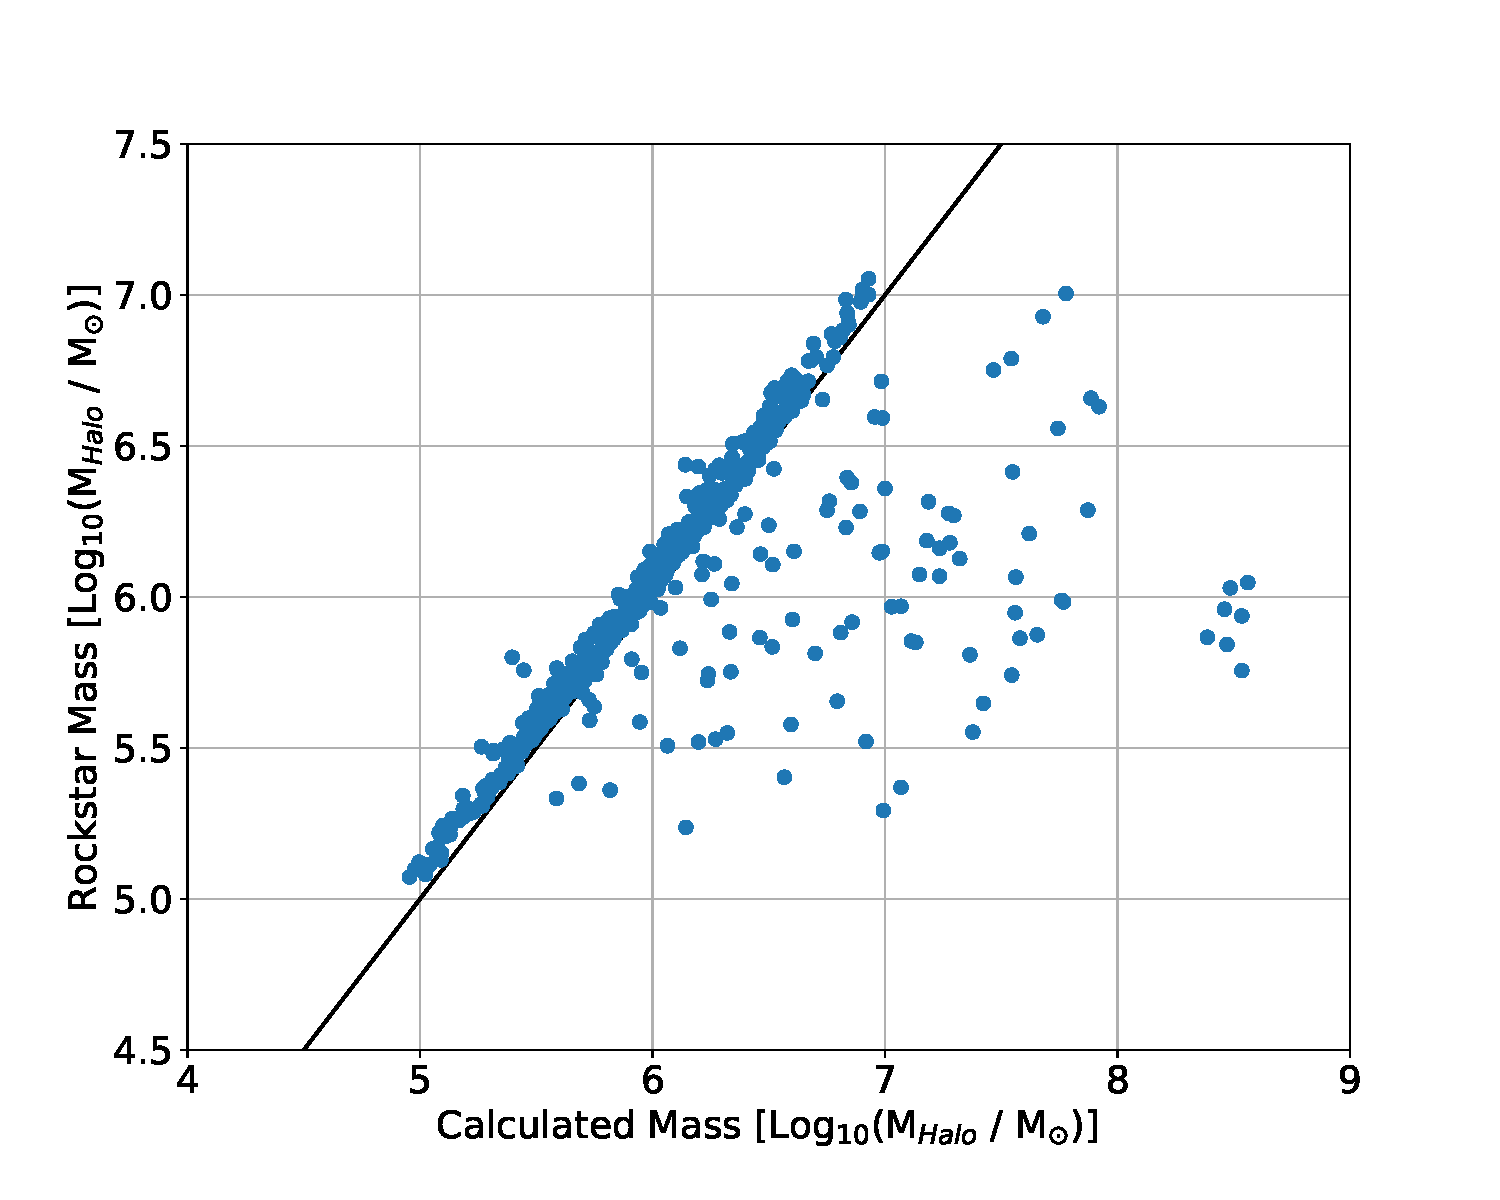
\includegraphics[width=\textwidth,height=\textheight,keepaspectratio]{images/compare_halo_mass.pdf}
    \label{fig:compare_mass}
\end{figure}

-Exclusion of atomic cooling haloes - we excluded these because of a bug in our code... how to explain this without simply saying that?

-Fraction of halos that halo Pop III stars forming outside the halos: Turns out I was not able to get this data as easily as I thought. I am going to quickly run through my script and find the P3 stars in each dataset which are not in halos.

\begin{referee}
Minor comments:

The authors should state at one point in the paper for which properties they use comoving or physical units.
\end{referee}
This has been clarified at the end of the second paragraph in the Simulation Setup section.

\begin{referee}
Introduction:

The authors write that Pop III star formation is generally more massive. While a fraction of the community agrees with that, there is manifoldly cited work that finds low-mass Pop III progenitors, and the authors should not let that unmentioned, but also cite eg Stacy+16, Greif+11 and Clark+11.
\end{referee}
These studies have been mentioned and cited in the introcution.

\begin{referee}
The authors name a few processes for suppressing Pop III star formation. For completeness, they should also mention eg X-ray heating (citing eg Jeon+14).
\end{referee}
This study has been mentioned and cited in the introduction.

\begin{referee}
The authors cite the well-known study from Machacek+01. However, a more recent result would be from the study by Visbal+14, giving a lower mass limit. Since the authors find a lower mass limit than Machacek+01, it would be interesting to see how this compares to the lower mass limit from the more modern paper.
\end{referee}
We have included the $M_{\rm crit}$ function that Visbal+14 use in their study (their Equation 4) for a redshift of 20 as a solid purple line in Figure 10. It appears the Visbal+14 find similar masses as Machacek+01, and when comparing the Machacek+01 for our LWBG and the relation from Visbal+14 at z=20, Visbal+14 find higher halo masses overall.

\begin{referee}
Methods:

In Wise+12, three different environment regions are picked. Please provide more description on the rare peak simulation here and discuss why this one is appropriate in this context.
\end{referee}
RP stands for radiation pressure in Wise+12, not rare peak. The simulation is the same size as ours, and contains similar physics, including the radiation pressure and soft UV background, which is why we reference it here. The differences are the inclusion of H2 self-shielding and updated cosmological parameters.
 
\begin{referee}
The initialization at z=130 is very late. I am aware that it is impossible to repeat this simulation starting at an earlier redshift, but would advise for future work.
\end{referee}

In hindsight, we agree that we initialized the simulation too late, even with 2nd order Lagrangian perturbation theory.  The maximum baryon overdensity is 1.64$\bar{\rho}_{\rm b}$, and the maximum DM particle displacement is 2.5 $\times$ (cell width).  In future studies, we will start at earlier times when the evolution is solidly in the linear regime.  We thank the referee for pointing this out.

\begin{referee}
Why do the authors pick a non-zero metalicity threshold for Pop III star formation? How many Pop III stars form between Z=0 and Z=5e-6 Z\_sol?
\end{referee}

We chose this metallicity threshold based on the work of Omukai et al. (2005), Schneider et al. (2006), who found that dust cooling was efficient enough above this metallicity to induce low-mass star formation. About 10\% of Pop III stars form with metallicities between zero and $5 \times 10^{-6} Z_\odot$.  Stars only obtain this extremely low (non-zero) metallicity when metal mixing is incomplete.  This usually occurs when a blastwave is mixing into a nearby halo, and the core collapses before it can fully mix.  Because of the randomness of the IMF sampling and errors from numerical diffusion and other solvers, we do not place great emphasis on stars in this metallicity range.  It is unclear what would be the actual stellar metallicity when it reaches main sequence, given our 0.1 proper pc resolution.  We have made a note of this in Section 2.2.1.

\begin{referee}
What is the physical motivation for a density threshold of 1.e6/cc? Is there convergence?
\end{referee}

Our choice was motivated by both previous work and our refinement strategy rather than convergence. Previous work (e.g. O'Shea et al. 2007; Yoshida et al. 2007) and later groups (e.g. Hirano et al. 2015) have shown that the number density is $\sim 10^6 \cubecm$ at our resolution limit of $0.09$ proper pc at $z=10$.  Secondly, we chose this threshold to be similar to the density that would trigger another level of AMR past our maximum level of 12 (dx = 0.09 proper pc at $z=10$).  At these scales, the grid is primarily refined from the Jeans length criterion, which is resolved by at least 8 cells.  Solving for the density in the Jeans length equation, given a typical temperature $T=300$~K with primordial cooling and a Jeans Length of $8 \times \textrm{dx}$, we obtain a number density $n = 5.7 \times 10^4 \cubecm$.  This number density does not exactly match the chosen density criterion because some oversight when setting up the simulation.  In the case where the density SF criterion is larger than $n$, the gas will continue to condense on a faster timescale than its surroundings.  Thus we are confident that this slight mismatch does not affect our results.

We have added the AMR refinement criteria to Section 2.1 and our motivation to this threshold to Section 2.2.1.

\begin{referee}
Similarly, why do the authors chose a H2 fraction of 1.e-3? (Is is a mass fraction or a number fraction?) How many Pop III stars do not form because of this threshold?
\end{referee}

We chose this critical H$_2$ fraction to match with the values found in previous work (e.g. Yoshida et al. 2007; Omukai et al. 2010) at the density threshold of $10^6 \cubecm$.  It is a number fraction.  We have added to Section 2.2.1 to reflect this detail.

In our original formulation (Abel et al. 2007), we implemented this restriction to avoid spurious star particle formation in D-type ionization fronts that can meet all of the other criteria.  But in the presence of an extremely strong Lyman-Werner flux from a nearby ($\sim$1 pc) star, star formation is unlikely to occur in the shell because it is irradiated and not self-gravitating. The last question is an interesting question, but it is difficult to determine because these conditions (high density but low H$_2$ fractions) are short-lived just after star formation.  Thus we cannot give a definite answer to it, but from the original formulation, we would estimate that the number of Pop III stars would increase by a factor of several with multiple cells in the quasi-spherical ionization front triggering star particle formation.  Because of these uncertainties, we have not added any of these details to the manuscript.

\begin{referee}
Do the authors set fixed mass limits to the IMF and if yes, which are they?  If not, which is the highest / lowest mass they find in their random sampling?  And which fraction of the Pop III stars in the simulation end up as type II SNe / BHs / PISN?
\end{referee}
We do set fixed mass limits, between 1 and 300 $M_{\odot}$. We have added this detail in section 2.2.1.  

59, 36, and 5 per cent of Pop III stars become Type II SN, black holes with no SN, and PISNe respectively. This detail has been added in section 2.2.1.

\begin{referee}
One effect than can weaken the shielding is shifting out of the Lyman-Werner resonance lines (see Hartwig+15). I am wondering how much this would affect the study presented here.
\end{referee}
-Would like to discuss this more in detail with John.

\begin{referee}
In Figure 1, please mention in the caption or at the top / bottom of the left axis that a shielding factor of 1 corresponds to no shielding and a shielding factor of 0 corresponds to high shielding, as these nomenclatures are not immediately understandable for the reader.
\end{referee}
This is a tricky detail, and has been added to the caption of Figure 1.

\begin{referee}
The analytic calculation of the shielding factor is a nice property of the paper. However, assuming a constant H2 fraction seems not appropriate. Please repeat this exercise for a more realistic halo profile, which could be found in the simulations or in the literature, eg by Machacek+01 themselves.
\end{referee}
This is a good point, and the plot has been adjusted accordingly. The halo profiles from O'Shea and Norman 2007 are now being used as the \hh{} fraction as a function of radius. The plot now shows that the shielding factor increases as a function of mass, since at larger radii, there is less \hh{}, resulting in a less effective \hh{} shield. The overall take away of the plot has not changed. 

\begin{referee}
Results:

Figure 2 is quite empty, it would be useful to include the halo mass function of the earliest Pop III formation redshift with its analytic prediction. In addition, the authors could provide a line or an arrow to show their halo mass resolution limit.
\end{referee}
We have added a vertical line at $10^5 M_{\odot}$ to show our halo mass resolution limit. This detail has also been added to the caption.

-The HMF at z=20 is overshooting the analytic estimate. Need to get together with John to see why. 

\begin{referee}
Figure 3 looks very nice. It would be helpful if an additional line that only 
provides the global LWBG (in units of J21) was included.
\end{referee}
Thank you for your comment. The global LWBG has been added as a red dashed line. More detail about the LW background (solid red line) has also been added.

\begin{referee}
The authors find no correlation between the host halo mass and the Lyman-Werner background intensity. However, they only look at the LWBG flux at the time of Pop III formation - is there maybe a correlation between the time integrated LW flux?
\end{referee}
While the time integrated LW flux would be interesting to follow, and may provide some further insight to what we are exploring, this would be difficult to calculate. It would require constant tracking of halos through time to calculate the time integrated LW flux. 

\begin{referee}
Figures 7 and 8 show very nice histograms as an additional panel on the right.  I suggest to include a histogram on the spread of the creation time in Figure 9 similar to Figures 7 and 8.
\end{referee}
The side histogram has been added to Figure 9. 

\begin{referee}
Discussion:

The authors give three reasons for the halo mass spread. Can they estimate which of the three processes (BH formation, dynamical heating and temporal LWBG fluctuations) is responsible for the spread by which fraction?
\end{referee}

This is an interesting question, but it is outside the scope of this paper.  It most likely depends on the large-scale environment, halo mass accretion history, and halo star formation history, but how these factors affect each other is unclear.  In practice, it would be difficult to determine the relative importance of dynamical heating and temporal LWBG fluctuations because of the time variations in the heating rate and suppression of H$_2$ cooling.  Because of these reasons, we do not give any estimates in the discussion.

The occurrence of BH formation and no metal enrichment depends on the chosen Pop III IMF, and we have addressed in an earlier answer and noted this fraction in the discussion.

\begin{referee}
One of the most extensive studies on over 1000 minihaloes was performed by Hirano+15, who also include a Lyman-Werner background. Their work should be put in comparison as well.
\end{referee}
This study has been added and cited in the Comparison section.
-Should more be added?

\begin{referee}
In Figure 10, the result from Yoshida+03 is hard to see, maybe use a different symbol / colour.
\end{referee}
This has been adjusted. The point from Yoshida+03 is now a pentagon and is outlined in black, and all symbols have had their edges increased for visibility.

\begin{referee}
Since the authors study star formation in minihaloes, it would be appropriate to also mention Kitayama+04 and Schauer+15 for the Lyman-Werner escape fractions from minihaloes.
\end{referee}
These papers have been added and referenced in the first paragraph of the caveats section. 

\begin{referee}
The authors mention a few times that streaming velocities are another pathway of suppressing Pop III formation (also in the introduction). While they cite some older work, they however fail to compare to more recent work eg by Hirano+18 or Schauer+19 (who do perform a systematic study not only based on a few, single haloes).
\end{referee}
The Schauer+19 study has been added to the caveat section.

\end{document}
